\documentclass[11pt]{article}

\author{Brooke Mosby and Michael Hansen}
\title{Predictions for Movie Success}

\usepackage{blindtext}
\usepackage{graphicx}
\usepackage{tikz}
\usepackage{textcomp}
\usepackage{soul}


\usepackage{listings}
\usepackage{xcolor}
\definecolor{red}{cmyk}{0, 1.00, 0.62,0}
\definecolor{blue}{cmyk}{1.00, .34, .0 .02 }    % blue
\definecolor{green}{cmyk}{0.7, 0, 1.0, 0.09 }   % greenish
\definecolor{yellow}{cmyk}{0, 0.16, 1.0, 0}     % yellow
\definecolor{gray}{cmyk}{0, 0, 0, 0.65}         % gray
\definecolor{purple}{cmyk}{.333, .867, 0, .059}
\colorlet{codebase}{yellow!30!}
\colorlet{codekeyword}{blue}
\colorlet{codecomment}{green}
\colorlet{codestring}{red}
\lstset{
  language=Python,
  backgroundcolor=\color{codebase},   %\color[RGB]{250, 245, 182},
  tabsize=4,
  basewidth=.5em,
  rulecolor=\color{yellow},           %\color{black},
  basicstyle=\normalsize\ttfamily,    % code text size
  upquote=true,
  columns=fixed,
  extendedchars=true,
  breaklines=true,
  prebreak = \raisebox{0ex}[0ex][0ex]{\ensuremath{\hookleftarrow}},
  frame=lrtb,
  xleftmargin=5pt,
  xrightmargin=5pt,
  framesep=4pt,
  framerule=2pt,
  showtabs=false,
  showspaces=false,
  showstringspaces=false,
  keywordstyle=\color{codekeyword},   %\color[RGB]{42, 161, 152},
  commentstyle=\color{codecomment},   %\color[RGB]{108, 153, 8},
  stringstyle=\color{codestring},     %\color[RGB]{189, 78, 98},
  title=\lstname,
  captionpos=b,
  abovecaptionskip=-5pt,
  belowcaptionskip=-5pt,
  moredelim=[is][\color{black}]{<<}{>>},
  moredelim=[is][\color{red}]{<r<}{>r>},
  moredelim=[is][\color{blue}]{<b<}{>b>},
  moredelim=[is][\color{green}]{<g<}{>g>},
  moredelim=[is][\color{purple}]{<p<}{>p>},
  morekeywords={assert, bytes, self, super, with, as, yield, True, False, None, NotImplemented, BaseException, Exception, AssertionError, AttributeError, ImportError, IndexError, KeyError, KeyboardInterrupt, MemoryError, NameError, NotImplementedError, OSError, OverflowError, RecursionError, RuntimeError, StopIteration, SyntaxError, IndentationError, TabError, StandardError, SystemError, SystemExit, TypeError, ValueError, ZeroDivisionError, IOError, Warning, RuntimeWarning, FileExistsError, FileNotFoundError,
    SELECT, FROM, AS, INNER, JOIN, LEFT, OUTER, CROSS, ON, WHERE, CASE, IF,
    MIN, MAX, SUM, AVG, COUNT, TEXT, REAL
  }
}

    \usepackage[T1]{fontenc}
% Nicer default font (+ math font) than Computer Modern for most use cases
\usepackage{mathpazo}

% Basic figure setup, for now with no caption control since it's done
% automatically by Pandoc (which extracts ![](path) syntax from Markdown).
\usepackage{graphicx}
% We will generate all images so they have a width \maxwidth. This means
% that they will get their normal width if they fit onto the page, but
% are scaled down if they would overflow the margins.
\makeatletter
\def\maxwidth{\ifdim\Gin@nat@width>\linewidth\linewidth
	\else\Gin@nat@width\fi}
\makeatother
\let\Oldincludegraphics\includegraphics
% Set max figure width to be 80% of text width, for now hardcoded.
\renewcommand{\includegraphics}[1]{\Oldincludegraphics[width=.8\maxwidth]{#1}}
% Ensure that by default, figures have no caption (until we provide a
% proper Figure object with a Caption API and a way to capture that
% in the conversion process - todo).
\usepackage{caption}
\DeclareCaptionLabelFormat{nolabel}{}
\captionsetup{labelformat=nolabel}

\usepackage{adjustbox} % Used to constrain images to a maximum size 
\usepackage{xcolor} % Allow colors to be defined
\usepackage{enumerate} % Needed for markdown enumerations to work
\usepackage{geometry} % Used to adjust the document margins
\usepackage{amsmath} % Equations
\usepackage{amssymb} % Equations
\usepackage{textcomp} % defines textquotesingle
% Hack from http://tex.stackexchange.com/a/47451/13684:
\AtBeginDocument{%
	\def\PYZsq{\textquotesingle}% Upright quotes in Pygmentized code
}
\usepackage{upquote} % Upright quotes for verbatim code
\usepackage{eurosym} % defines \euro
\usepackage[mathletters]{ucs} % Extended unicode (utf-8) support
\usepackage[utf8x]{inputenc} % Allow utf-8 characters in the tex document
\usepackage{fancyvrb} % verbatim replacement that allows latex
\usepackage{grffile} % extends the file name processing of package graphics 
% to support a larger range 
% The hyperref package gives us a pdf with properly built
% internal navigation ('pdf bookmarks' for the table of contents,
% internal cross-reference links, web links for URLs, etc.)
\usepackage{hyperref}
\usepackage{longtable} % longtable support required by pandoc >1.10
\usepackage{booktabs}  % table support for pandoc > 1.12.2
\usepackage[inline]{enumitem} % IRkernel/repr support (it uses the enumerate* environment)
\usepackage[normalem]{ulem} % ulem is needed to support strikethroughs (\sout)
% normalem makes italics be italics, not underlines




% Colors for the hyperref package
\definecolor{urlcolor}{rgb}{0,.145,.698}
\definecolor{linkcolor}{rgb}{.71,0.21,0.01}
\definecolor{citecolor}{rgb}{.12,.54,.11}

% ANSI colors
\definecolor{ansi-black}{HTML}{3E424D}
\definecolor{ansi-black-intense}{HTML}{282C36}
\definecolor{ansi-red}{HTML}{E75C58}
\definecolor{ansi-red-intense}{HTML}{B22B31}
\definecolor{ansi-green}{HTML}{00A250}
\definecolor{ansi-green-intense}{HTML}{007427}
\definecolor{ansi-yellow}{HTML}{DDB62B}
\definecolor{ansi-yellow-intense}{HTML}{B27D12}
\definecolor{ansi-blue}{HTML}{208FFB}
\definecolor{ansi-blue-intense}{HTML}{0065CA}
\definecolor{ansi-magenta}{HTML}{D160C4}
\definecolor{ansi-magenta-intense}{HTML}{A03196}
\definecolor{ansi-cyan}{HTML}{60C6C8}
\definecolor{ansi-cyan-intense}{HTML}{258F8F}
\definecolor{ansi-white}{HTML}{C5C1B4}
\definecolor{ansi-white-intense}{HTML}{A1A6B2}

% commands and environments needed by pandoc snippets
% extracted from the output of `pandoc -s`
\providecommand{\tightlist}{%
	\setlength{\itemsep}{0pt}\setlength{\parskip}{0pt}}
\DefineVerbatimEnvironment{Highlighting}{Verbatim}{commandchars=\\\{\}}
% Add ',fontsize=\small' for more characters per line
\newenvironment{Shaded}{}{}
\newcommand{\KeywordTok}[1]{\textcolor[rgb]{0.00,0.44,0.13}{\textbf{{#1}}}}
\newcommand{\DataTypeTok}[1]{\textcolor[rgb]{0.56,0.13,0.00}{{#1}}}
\newcommand{\DecValTok}[1]{\textcolor[rgb]{0.25,0.63,0.44}{{#1}}}
\newcommand{\BaseNTok}[1]{\textcolor[rgb]{0.25,0.63,0.44}{{#1}}}
\newcommand{\FloatTok}[1]{\textcolor[rgb]{0.25,0.63,0.44}{{#1}}}
\newcommand{\CharTok}[1]{\textcolor[rgb]{0.25,0.44,0.63}{{#1}}}
\newcommand{\StringTok}[1]{\textcolor[rgb]{0.25,0.44,0.63}{{#1}}}
\newcommand{\CommentTok}[1]{\textcolor[rgb]{0.38,0.63,0.69}{\textit{{#1}}}}
\newcommand{\OtherTok}[1]{\textcolor[rgb]{0.00,0.44,0.13}{{#1}}}
\newcommand{\AlertTok}[1]{\textcolor[rgb]{1.00,0.00,0.00}{\textbf{{#1}}}}
\newcommand{\FunctionTok}[1]{\textcolor[rgb]{0.02,0.16,0.49}{{#1}}}
\newcommand{\RegionMarkerTok}[1]{{#1}}
\newcommand{\ErrorTok}[1]{\textcolor[rgb]{1.00,0.00,0.00}{\textbf{{#1}}}}
\newcommand{\NormalTok}[1]{{#1}}

% Additional commands for more recent versions of Pandoc
\newcommand{\ConstantTok}[1]{\textcolor[rgb]{0.53,0.00,0.00}{{#1}}}
\newcommand{\SpecialCharTok}[1]{\textcolor[rgb]{0.25,0.44,0.63}{{#1}}}
\newcommand{\VerbatimStringTok}[1]{\textcolor[rgb]{0.25,0.44,0.63}{{#1}}}
\newcommand{\SpecialStringTok}[1]{\textcolor[rgb]{0.73,0.40,0.53}{{#1}}}
\newcommand{\ImportTok}[1]{{#1}}
\newcommand{\DocumentationTok}[1]{\textcolor[rgb]{0.73,0.13,0.13}{\textit{{#1}}}}
\newcommand{\AnnotationTok}[1]{\textcolor[rgb]{0.38,0.63,0.69}{\textbf{\textit{{#1}}}}}
\newcommand{\CommentVarTok}[1]{\textcolor[rgb]{0.38,0.63,0.69}{\textbf{\textit{{#1}}}}}
\newcommand{\VariableTok}[1]{\textcolor[rgb]{0.10,0.09,0.49}{{#1}}}
\newcommand{\ControlFlowTok}[1]{\textcolor[rgb]{0.00,0.44,0.13}{\textbf{{#1}}}}
\newcommand{\OperatorTok}[1]{\textcolor[rgb]{0.40,0.40,0.40}{{#1}}}
\newcommand{\BuiltInTok}[1]{{#1}}
\newcommand{\ExtensionTok}[1]{{#1}}
\newcommand{\PreprocessorTok}[1]{\textcolor[rgb]{0.74,0.48,0.00}{{#1}}}
\newcommand{\AttributeTok}[1]{\textcolor[rgb]{0.49,0.56,0.16}{{#1}}}
\newcommand{\InformationTok}[1]{\textcolor[rgb]{0.38,0.63,0.69}{\textbf{\textit{{#1}}}}}
\newcommand{\WarningTok}[1]{\textcolor[rgb]{0.38,0.63,0.69}{\textbf{\textit{{#1}}}}}


% Define a nice break command that doesn't care if a line doesn't already
% exist.
\def\br{\hspace*{\fill} \\* }
% Math Jax compatability definitions
\def\gt{>}
\def\lt{<}





% Pygments definitions

\makeatletter
\def\PY@reset{\let\PY@it=\relax \let\PY@bf=\relax%
	\let\PY@ul=\relax \let\PY@tc=\relax%
	\let\PY@bc=\relax \let\PY@ff=\relax}
\def\PY@tok#1{\csname PY@tok@#1\endcsname}
\def\PY@toks#1+{\ifx\relax#1\empty\else%
	\PY@tok{#1}\expandafter\PY@toks\fi}
\def\PY@do#1{\PY@bc{\PY@tc{\PY@ul{%
				\PY@it{\PY@bf{\PY@ff{#1}}}}}}}
\def\PY#1#2{\PY@reset\PY@toks#1+\relax+\PY@do{#2}}

\expandafter\def\csname PY@tok@w\endcsname{\def\PY@tc##1{\textcolor[rgb]{0.73,0.73,0.73}{##1}}}
\expandafter\def\csname PY@tok@c\endcsname{\let\PY@it=\textit\def\PY@tc##1{\textcolor[rgb]{0.25,0.50,0.50}{##1}}}
\expandafter\def\csname PY@tok@cp\endcsname{\def\PY@tc##1{\textcolor[rgb]{0.74,0.48,0.00}{##1}}}
\expandafter\def\csname PY@tok@k\endcsname{\let\PY@bf=\textbf\def\PY@tc##1{\textcolor[rgb]{0.00,0.50,0.00}{##1}}}
\expandafter\def\csname PY@tok@kp\endcsname{\def\PY@tc##1{\textcolor[rgb]{0.00,0.50,0.00}{##1}}}
\expandafter\def\csname PY@tok@kt\endcsname{\def\PY@tc##1{\textcolor[rgb]{0.69,0.00,0.25}{##1}}}
\expandafter\def\csname PY@tok@o\endcsname{\def\PY@tc##1{\textcolor[rgb]{0.40,0.40,0.40}{##1}}}
\expandafter\def\csname PY@tok@ow\endcsname{\let\PY@bf=\textbf\def\PY@tc##1{\textcolor[rgb]{0.67,0.13,1.00}{##1}}}
\expandafter\def\csname PY@tok@nb\endcsname{\def\PY@tc##1{\textcolor[rgb]{0.00,0.50,0.00}{##1}}}
\expandafter\def\csname PY@tok@nf\endcsname{\def\PY@tc##1{\textcolor[rgb]{0.00,0.00,1.00}{##1}}}
\expandafter\def\csname PY@tok@nc\endcsname{\let\PY@bf=\textbf\def\PY@tc##1{\textcolor[rgb]{0.00,0.00,1.00}{##1}}}
\expandafter\def\csname PY@tok@nn\endcsname{\let\PY@bf=\textbf\def\PY@tc##1{\textcolor[rgb]{0.00,0.00,1.00}{##1}}}
\expandafter\def\csname PY@tok@ne\endcsname{\let\PY@bf=\textbf\def\PY@tc##1{\textcolor[rgb]{0.82,0.25,0.23}{##1}}}
\expandafter\def\csname PY@tok@nv\endcsname{\def\PY@tc##1{\textcolor[rgb]{0.10,0.09,0.49}{##1}}}
\expandafter\def\csname PY@tok@no\endcsname{\def\PY@tc##1{\textcolor[rgb]{0.53,0.00,0.00}{##1}}}
\expandafter\def\csname PY@tok@nl\endcsname{\def\PY@tc##1{\textcolor[rgb]{0.63,0.63,0.00}{##1}}}
\expandafter\def\csname PY@tok@ni\endcsname{\let\PY@bf=\textbf\def\PY@tc##1{\textcolor[rgb]{0.60,0.60,0.60}{##1}}}
\expandafter\def\csname PY@tok@na\endcsname{\def\PY@tc##1{\textcolor[rgb]{0.49,0.56,0.16}{##1}}}
\expandafter\def\csname PY@tok@nt\endcsname{\let\PY@bf=\textbf\def\PY@tc##1{\textcolor[rgb]{0.00,0.50,0.00}{##1}}}
\expandafter\def\csname PY@tok@nd\endcsname{\def\PY@tc##1{\textcolor[rgb]{0.67,0.13,1.00}{##1}}}
\expandafter\def\csname PY@tok@s\endcsname{\def\PY@tc##1{\textcolor[rgb]{0.73,0.13,0.13}{##1}}}
\expandafter\def\csname PY@tok@sd\endcsname{\let\PY@it=\textit\def\PY@tc##1{\textcolor[rgb]{0.73,0.13,0.13}{##1}}}
\expandafter\def\csname PY@tok@si\endcsname{\let\PY@bf=\textbf\def\PY@tc##1{\textcolor[rgb]{0.73,0.40,0.53}{##1}}}
\expandafter\def\csname PY@tok@se\endcsname{\let\PY@bf=\textbf\def\PY@tc##1{\textcolor[rgb]{0.73,0.40,0.13}{##1}}}
\expandafter\def\csname PY@tok@sr\endcsname{\def\PY@tc##1{\textcolor[rgb]{0.73,0.40,0.53}{##1}}}
\expandafter\def\csname PY@tok@ss\endcsname{\def\PY@tc##1{\textcolor[rgb]{0.10,0.09,0.49}{##1}}}
\expandafter\def\csname PY@tok@sx\endcsname{\def\PY@tc##1{\textcolor[rgb]{0.00,0.50,0.00}{##1}}}
\expandafter\def\csname PY@tok@m\endcsname{\def\PY@tc##1{\textcolor[rgb]{0.40,0.40,0.40}{##1}}}
\expandafter\def\csname PY@tok@gh\endcsname{\let\PY@bf=\textbf\def\PY@tc##1{\textcolor[rgb]{0.00,0.00,0.50}{##1}}}
\expandafter\def\csname PY@tok@gu\endcsname{\let\PY@bf=\textbf\def\PY@tc##1{\textcolor[rgb]{0.50,0.00,0.50}{##1}}}
\expandafter\def\csname PY@tok@gd\endcsname{\def\PY@tc##1{\textcolor[rgb]{0.63,0.00,0.00}{##1}}}
\expandafter\def\csname PY@tok@gi\endcsname{\def\PY@tc##1{\textcolor[rgb]{0.00,0.63,0.00}{##1}}}
\expandafter\def\csname PY@tok@gr\endcsname{\def\PY@tc##1{\textcolor[rgb]{1.00,0.00,0.00}{##1}}}
\expandafter\def\csname PY@tok@ge\endcsname{\let\PY@it=\textit}
\expandafter\def\csname PY@tok@gs\endcsname{\let\PY@bf=\textbf}
\expandafter\def\csname PY@tok@gp\endcsname{\let\PY@bf=\textbf\def\PY@tc##1{\textcolor[rgb]{0.00,0.00,0.50}{##1}}}
\expandafter\def\csname PY@tok@go\endcsname{\def\PY@tc##1{\textcolor[rgb]{0.53,0.53,0.53}{##1}}}
\expandafter\def\csname PY@tok@gt\endcsname{\def\PY@tc##1{\textcolor[rgb]{0.00,0.27,0.87}{##1}}}
\expandafter\def\csname PY@tok@err\endcsname{\def\PY@bc##1{\setlength{\fboxsep}{0pt}\fcolorbox[rgb]{1.00,0.00,0.00}{1,1,1}{\strut ##1}}}
\expandafter\def\csname PY@tok@kc\endcsname{\let\PY@bf=\textbf\def\PY@tc##1{\textcolor[rgb]{0.00,0.50,0.00}{##1}}}
\expandafter\def\csname PY@tok@kd\endcsname{\let\PY@bf=\textbf\def\PY@tc##1{\textcolor[rgb]{0.00,0.50,0.00}{##1}}}
\expandafter\def\csname PY@tok@kn\endcsname{\let\PY@bf=\textbf\def\PY@tc##1{\textcolor[rgb]{0.00,0.50,0.00}{##1}}}
\expandafter\def\csname PY@tok@kr\endcsname{\let\PY@bf=\textbf\def\PY@tc##1{\textcolor[rgb]{0.00,0.50,0.00}{##1}}}
\expandafter\def\csname PY@tok@bp\endcsname{\def\PY@tc##1{\textcolor[rgb]{0.00,0.50,0.00}{##1}}}
\expandafter\def\csname PY@tok@fm\endcsname{\def\PY@tc##1{\textcolor[rgb]{0.00,0.00,1.00}{##1}}}
\expandafter\def\csname PY@tok@vc\endcsname{\def\PY@tc##1{\textcolor[rgb]{0.10,0.09,0.49}{##1}}}
\expandafter\def\csname PY@tok@vg\endcsname{\def\PY@tc##1{\textcolor[rgb]{0.10,0.09,0.49}{##1}}}
\expandafter\def\csname PY@tok@vi\endcsname{\def\PY@tc##1{\textcolor[rgb]{0.10,0.09,0.49}{##1}}}
\expandafter\def\csname PY@tok@vm\endcsname{\def\PY@tc##1{\textcolor[rgb]{0.10,0.09,0.49}{##1}}}
\expandafter\def\csname PY@tok@sa\endcsname{\def\PY@tc##1{\textcolor[rgb]{0.73,0.13,0.13}{##1}}}
\expandafter\def\csname PY@tok@sb\endcsname{\def\PY@tc##1{\textcolor[rgb]{0.73,0.13,0.13}{##1}}}
\expandafter\def\csname PY@tok@sc\endcsname{\def\PY@tc##1{\textcolor[rgb]{0.73,0.13,0.13}{##1}}}
\expandafter\def\csname PY@tok@dl\endcsname{\def\PY@tc##1{\textcolor[rgb]{0.73,0.13,0.13}{##1}}}
\expandafter\def\csname PY@tok@s2\endcsname{\def\PY@tc##1{\textcolor[rgb]{0.73,0.13,0.13}{##1}}}
\expandafter\def\csname PY@tok@sh\endcsname{\def\PY@tc##1{\textcolor[rgb]{0.73,0.13,0.13}{##1}}}
\expandafter\def\csname PY@tok@s1\endcsname{\def\PY@tc##1{\textcolor[rgb]{0.73,0.13,0.13}{##1}}}
\expandafter\def\csname PY@tok@mb\endcsname{\def\PY@tc##1{\textcolor[rgb]{0.40,0.40,0.40}{##1}}}
\expandafter\def\csname PY@tok@mf\endcsname{\def\PY@tc##1{\textcolor[rgb]{0.40,0.40,0.40}{##1}}}
\expandafter\def\csname PY@tok@mh\endcsname{\def\PY@tc##1{\textcolor[rgb]{0.40,0.40,0.40}{##1}}}
\expandafter\def\csname PY@tok@mi\endcsname{\def\PY@tc##1{\textcolor[rgb]{0.40,0.40,0.40}{##1}}}
\expandafter\def\csname PY@tok@il\endcsname{\def\PY@tc##1{\textcolor[rgb]{0.40,0.40,0.40}{##1}}}
\expandafter\def\csname PY@tok@mo\endcsname{\def\PY@tc##1{\textcolor[rgb]{0.40,0.40,0.40}{##1}}}
\expandafter\def\csname PY@tok@ch\endcsname{\let\PY@it=\textit\def\PY@tc##1{\textcolor[rgb]{0.25,0.50,0.50}{##1}}}
\expandafter\def\csname PY@tok@cm\endcsname{\let\PY@it=\textit\def\PY@tc##1{\textcolor[rgb]{0.25,0.50,0.50}{##1}}}
\expandafter\def\csname PY@tok@cpf\endcsname{\let\PY@it=\textit\def\PY@tc##1{\textcolor[rgb]{0.25,0.50,0.50}{##1}}}
\expandafter\def\csname PY@tok@c1\endcsname{\let\PY@it=\textit\def\PY@tc##1{\textcolor[rgb]{0.25,0.50,0.50}{##1}}}
\expandafter\def\csname PY@tok@cs\endcsname{\let\PY@it=\textit\def\PY@tc##1{\textcolor[rgb]{0.25,0.50,0.50}{##1}}}

\def\PYZbs{\char`\\}
\def\PYZus{\char`\_}
\def\PYZob{\char`\{}
\def\PYZcb{\char`\}}
\def\PYZca{\char`\^}
\def\PYZam{\char`\&}
\def\PYZlt{\char`\<}
\def\PYZgt{\char`\>}
\def\PYZsh{\char`\#}
\def\PYZpc{\char`\%}
\def\PYZdl{\char`\$}
\def\PYZhy{\char`\-}
\def\PYZsq{\char`\'}
\def\PYZdq{\char`\"}
\def\PYZti{\char`\~}
% for compatibility with earlier versions
\def\PYZat{@}
\def\PYZlb{[}
\def\PYZrb{]}
\makeatother


% Exact colors from NB
\definecolor{incolor}{rgb}{0.0, 0.0, 0.5}
\definecolor{outcolor}{rgb}{0.545, 0.0, 0.0}




% Prevent overflowing lines due to hard-to-break entities
\sloppy 
% Setup hyperref package
\hypersetup{
	breaklinks=true,  % so long urls are correctly broken across lines
	colorlinks=true,
	urlcolor=urlcolor,
	linkcolor=linkcolor,
	citecolor=citecolor,
}
% Slightly bigger margins than the latex defaults












%code box \begin{lstlisting} ... \end{lstlisting}
\begin{document}
\maketitle

\hl{Case Study, Monday we review it all}

\hypertarget{abstract}{%
\begin{abstract}\label{abstract}}
Cinema has become one of the highest profiting industries over the past
century. The total box office revenue in North America alone amounted to
\$11.38 billion in 2016. With the possibility of great success, there is
also a large risk of financial failure. This machine learning project is
motivated by answering the question of what makes a movie successful. There
are plenty of quantative data available for movies, such as the movies'
budget, the release date, ratings etc., but in this analysis an attempt
will be made to quantify movie information that is less measurable and
then predict movie success.
\end{abstract}

%\begin{lstlisting}
%import pandas as pd
%import numpy as np
%import networkx as nx
%from sklearn.ensemble import RandomForestRegressor as RFR
%from sklearn.model_selection import train_test_split as tts
%from sklearn.model_selection import cross_val_score, GridSearchCV
%from sklearn import linear_model
%from sklearn.decomposition import PCA
%from sklearn.pipeline import Pipeline
%from catboost import Pool, CatBoostRegressor
%import re, json, requests, seaborn, warnings
%warnings.filterwarnings( 'ignore' )
%from bs4 import BeautifulSoup
%from matplotlib import pyplot as plt, rcParams
%%matplotlib inline
%from selenium import webdriver
%from selenium.webdriver.common.keys import Keys
%from selenium.common.exceptions import NoSuchElementException
%from ipyparallel import Client
%import time
%\end{lstlisting}



\hypertarget{introduction}{%
	\section{Introduction}\label{introduction}}

Research has been done to determine what aspects of a movie make it more
successful; however, much of this research is contradictory. The
research paper ``Early Predictions of Movie Success: the Who, What, and
When of Profitability''$^{[1]}$ states movies with a motion picture content
rating `R' will likely have lower profits, whereas the research paper
``What Makes A Great Movie?''$^{[2]}$ states a motion picture content rating `R'
will have higher a box-office. Both papers analyzed thousands of movies,
but came to opposite conclusions. Some variables used to predict movie
success in these studies, included budget, motion picture content
rating, and actor popularity.\\
Based on these previous models, the dataset used includes movie
title length, run-time, motion picture content rating, director, genre,
release date, actors, actor network scores, budget, opening weekend box-office revenue, and a list of other predictor variables. A network of actors was created to observe the impact certain popular actors and combinations of actors had on the success. Movie success will be
determined by whether or not the movie turns a profit.

\hypertarget{data-scraped-downloaded-cleaned-engineered}{%
	\section{Data Scraped, Downloaded, Cleaned \&
		Engineered}\label{data-scraped-downloaded-cleaned-engineered}}

\hypertarget{beginning-dataset}{%
	\subsection{Dataset}\label{beginning-dataset}}

A beginning dataset was downloaded from IMDb with 10,000 movies, each
entry containing \texttt{Title, URL} (on IMDb)\texttt{, IMDb Rating, Runtime} (in minutes)\texttt{, Year,
Genres, Num Votes, Release Date, Directors.} From this dataset,
additional information on the \texttt{Budget, Gross, Opening
Weekend, Actors\_0-Actors\_9, Oscar Nominations, Oscars Wins, Other Nominations, Other Wins, Meta Score, and Content Rating} was
scraped and cleaned. The data points were collected from IMDb, which
is a reputable source for information, according to their website,

\begin{quote}
	``We [IMDb] actively gather information from and verify items with
	studios and filmmakers''$^{[3]}$.
\end{quote}

\hypertarget{cleaning-data}{%
	\subsection{Cleaning Data}\label{cleaning-data}}

The data set was completed after gathering each data point, although the
information is not clean or uniform. The first step to clean the data
was to remove all commas across each column in the DataFrame.
Removing commas made it easier to convert monetary amounts to integer values.
Next, each date in the \texttt{Release Date} column was changed to a pandas date
object, which simplified any calculations that rely on the release
date of the movie. Each monetary value was converted into an integer in US dollar amounts. Each unique genre was made into a column
with a true or false boolean for each movie entry. Using booleans instead of categorical data causes less problems when implementing regression.

\hypertarget{feature-engineering}{%
	\subsection{Feature Engineering}\label{feature-engineering}}

To resolve the disagreement in monetary amounts due to
inflation, a dataset containing the CPI for each year from 1913 was
used to adjust the values. The CPI (Consumer Price Index)
describes the amount of purchasing power the average consumer has. For example, the purchasing power of 1 US dollar in January of 1913 is equivalent to approximately 24.69 US dollars in January of 2017. The
length of the movie title was added, and a NetworkX graph of all
actors was made. This was used to add a column describing the total edge weight for actors in each movie.
\hypertarget{actor-network}{%
	\subsubsection{Actor Network}\label{actor-network}}

Using the Python library NetworkX, a network of actors was made to help determine the success of a
movie. Each node in the network is an actor that has appeared in a
movie, and that actor node has an edge to another actor node if
they appeared in a movie together. The weights on each edge
correspond to the amount of movies the two actors appeared in together. In the example below, edges with Johnny Depp having weight 1 were ignored. The other nodes and edges demonstrate how the graph was assembled, actor to actor with the edge weight being the number of movies they appear in together according to the dataset used.

\[
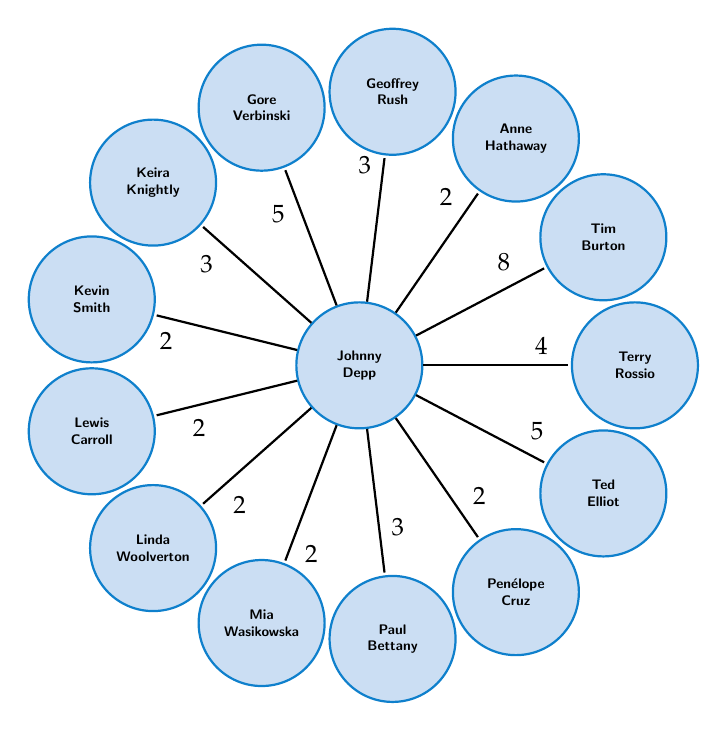
\begin{tikzpicture}[shorten >=1pt,thick]

\foreach [count=\i] \a/\t/\d in {2/Anne\\Hathaway/3.5, 3/Geoffrey\\Rush/3.5, 4/Gore\\Verbinski/3.5, 5/Keira\\Knightly/3.5, 6/Kevin\\Smith/3.5, 7/Lewis\\Carroll/3.5, 8/Linda\\Woolverton/3.5, 9/Mia\\Wasikowska/3.5, 10/Paul\\Bettany/3.5, 11/Penélope\\Cruz/3.5, 12/Ted\\Elliot/3.5, 13/Terry\\Rossio/3.5, 1/Tim\\Burton/3.5, 0/Johnny\\Depp/0}
\draw (\a*360/13: \d cm) node[circle,draw=blue,fill=blue!20!,font=\sffamily\tiny\bfseries,align=center,minimum size=1.6cm] (v\i)  {\t};

\foreach \i/\j/\w in {14/1/2,14/2/3,14/3/5,14/4/3,14/5/2,14/6/2,14/7/2,14/8/2,14/9/3,14/10/2,14/11/5,14/12/4,14/13/8}
\draw [black,thick]  (v\i) edge node [font=\small,pos=.8,auto] {\w} (v\j);


\end{tikzpicture}
\]

\hypertarget{final-dataset}{%
	\subsection{Final Dataset}\label{final-dataset}}
The most significant variables in the final dataset are \texttt{Title, Length of Title,
Content Rating, Runtime (mins), IMDb Rating, Genres, Content Rating, Meta
Score, Oscar Nominations, Oscar Wins, Other Nominations, Other
Wins, Director, Release Date, Budget, Budget Adjusted, Opening Weekend, Opening Weekend Adjusted, Gross, Gross Adjusted, Profit, Profit Adjusted, Profit Bool, Directors Prev Total Profit, Actor\_0-Actor\_9} (the top ten actors in each movie), and \texttt{Actor Weights.} A separate
NetworkX object holds the actor nodes and their connections. 




%\begin{lstlisting}
%df = pd.read_csv("Result_Data/total_engineered.csv",encoding = "ISO-8859-1")
%del df["Unnamed: 0"]
%df = df.fillna(df.mean())
%print(", ".join(list(df.columns)))
%\end{lstlisting}

%\begin{Verbatim}[commandchars=\\\{\}]
%Actor\_0, Actor\_1, Actor\_2, Actor\_3, Actor\_4, Actor\_5, Actor\_6, Actor\_7, Actor\_8,
%Actor\_9, Budget, Directors, Gross, IMDb Rating, Meta Score, Num Votes, Opening Weekend,
%Oscar Nominations, Oscar Wins, Other Nominations, Other Wins, Release Date, Runtime (mins),
%Title, Year, Genre: Short, Genre:  Comedy, Genre: Fantasy, Genre: Film-Noir, Genre: War,
%Genre: Musical, Genre:  Sport, Genre: Biography, Genre: Action, Genre:  Fantasy, Genre:  
%Animation, Genre:  Biography, Genre: Mystery, Genre:  Musical, Genre:  Romance, Genre: 
%Thriller, Genre:  Film-Noir, Genre:  History, Genre: Western, Genre: Drama, Genre: Sci-Fi,
%Genre:  Horror, Genre: Romance, Genre: Adventure, Genre:  Family, Genre:  Sci-Fi,
%Genre: Animation, Genre:  Music, Genre: Music, Genre: History, Genre:  Mystery, Genre: 
%Thriller, Genre: Comedy, Genre:  Crime, Genre: Horror, Genre:  Drama, Genre:  War, Genre: 
%Western, Genre:  Adventure, Genre: Family, Genre:  Action, Genre: Crime, Content Rating:
%PASSED, Content Rating: TV-MA, Content Rating: X, Content Rating: NC-17, Content Rating:
%TV-14, Content Rating: M, Content Rating: GP, Content Rating: TV-PG, Content Rating: PG,
%Content Rating: PG-13, Content Rating: G, Content Rating: NR, Content Rating: APPROVED,
%Content Rating: UNRATED, Content Rating: M/PG, Content Rating: TV-13, Content Rating: 
%NOT RATED, Content Rating: TV-G, Content Rating: R, Decade, Profit, Budget\_Adjusted,
%Gross\_Adjusted, Open\_Adjusted, Profit\_Adjusted, Profit\_Bool, Total Nominations,
%Total Wins, Length of Title, Directors Prev Number Movies, Directors Prev Total Profit,
%Directors Prev Mean Profit, Directors Prev Mean IMDb, Directors Prev Mean Meta, Directors 
%Prev Mean Num Votes, Directors Prev Mean Nominations, Directors Prev Mean Wins, Actor Weights
%\end{Verbatim}

%\begin{lstlisting}
%df_x = df[['Actor_0', 'Actor_1', 'Actor_2', 'Actor_3', 'Actor_4','Actor_5',
%		   'Actor_6', 'Actor_7', 'Actor_8', 'Actor_9', 'Budget',
%		   'Directors', 'Release Date', 'Runtime (mins)', 'Title', 'Year',
%		   'Genre: Short', 'Genre:  Comedy', 'Genre: Fantasy',
%		   'Genre: Film-Noir', 'Genre: War', 'Genre: Musical', 
%		   'Genre:  Sport', 'Genre: Biography', 'Genre: Action', 
%		   'Genre:  Fantasy', 'Genre:  Animation', 'Genre:  Biography',
%		   'Genre: Mystery', 'Genre:  Musical', 'Genre:  Romance', 
%		   'Genre: Thriller', 'Genre:  Film-Noir', 'Genre:  History',
%		   'Genre: Western', 'Genre: Drama', 'Genre: Sci-Fi', 
%		   'Genre:  Horror', 'Genre: Romance', 'Genre: Adventure',
%		   'Genre:  Family', 'Genre:  Sci-Fi', 'Genre: Animation',
%		   'Genre:  Music', 'Genre: Music', 'Genre: History',
%		   'Genre:  Mystery', 'Genre:  Thriller', 'Genre: Comedy',
%		   'Genre:  Crime', 'Genre: Horror', 'Genre:  Drama',
%		   'Genre:  War', 'Genre:  Western', 'Genre:  Adventure',
%		   'Genre: Family', 'Genre:  Action', 'Genre: Crime',
%		   'Content Rating: PASSED', 'Content Rating: TV-MA',
%		   'Content Rating: X', 'Content Rating: NC-17',
%		   'Content Rating: TV-14', 'Content Rating: M', 
%		   'Content Rating: GP', 'Content Rating: TV-PG',
%		   'Content Rating: PG', 'Content Rating: PG-13',
%		   'Content Rating: G', 'Content Rating: NR', 
%		   'Content Rating: APPROVED', 'Content Rating: UNRATED',
%		   'Content Rating: M/PG', 'Content Rating: TV-13',
%		   'Content Rating: NOT RATED', 'Content Rating: TV-G',
%		   'Content Rating: R','Decade', 'Budget_Adjusted',
%		   'Length of Title', 'Directors Prev Number Movies',
%		   'Directors Prev Mean Profit', 'Directors Prev Mean IMDb',
%		   'Directors Prev Mean Meta', 'Directors Prev Mean Num Votes',
%		   'Directors Prev Mean Nominations', 'Directors Prev Mean Wins',
%		   'Actor Weights']]
%df_y = df[['Gross', 'IMDb Rating', 'Meta Score', 'Num Votes',
%           'Oscar Nominations', 'Oscar Wins', 'Other Nominations',
%           'Other Wins','Profit','Gross_Adjusted',  'Profit_Adjusted',
%           'Profit_Bool', 'Total Nominations', 'Total Wins']]
%\end{lstlisting}

\hypertarget{methods}{%
	\section{Methods}\label{methods}}

Various supervised machine learning models are used to predict certain
characteristics of the movie that determine a movie's success. The
variables that our models attempt to predict are the movie's IMDb
rating, Metacritic Score, the number of votes it recieves on IMDb, the
number of Oscar nominations, the number of Oscar wins, the number of
other award nominations, the number of other award wins, the number of
total award nominations, the number of total award wins, gross, the
profit,the gross adjusted for inflation, the profit adjusted for
inflation, and finally whether or not a movie turned a profit. These
varaibles will hereon be referred to as the movies' independent
variables. For each model the data is split into a training and testing
set to determine how accurate each method proves.

\hypertarget{pca}{%
	\subsection{PCA}\label{pca}}

Principal Component Analysis (PCA) is used to reduce the dimensionality of the large dataset while retaining important information. For each Machine Learning model, PCA is used to reduce dimensionality to 10, 20, and 50 components, and then compared to find the best dimensionality. Because our dataset contains over 100 columns, PCA is essential for our models to avoid extremely costly computations and produce more accurate results.


%\begin{lstlisting}
%pca = PCA()
%df_x_temp = df_x.select_dtypes(include=['float64','int',
%            'bool']).astype('float')
%df_y_temp = df_y.select_dtypes(include=['float64','int',
%            'bool']).astype('float')
%tr_x, tt_x, tr_y, tt_y = tts(df_x_temp, df_y_temp, test_size = .2)
%
%def results(es_y1):
%	"""
%	Accepts a regression prediction for variables and prints 
%	accuracy values of prediction, so it is easier to digest.
%	Returns Nothing
%	"""
%	print("\nMovie Gross Average Percent Error:")
%	print((abs(es_y1[0:,0]-np.array(tt_y.astype(float))[0:,0])
%	      /abs(np.array(tt_y.astype(float))[0:,0])).mean()*100,"%")
%	print("\nIMDb Rating Average Percent Error:")
%	print((abs(es_y1[0:,1]-np.array(tt_y.astype(float))[0:,1])
%	     /abs(np.array(tt_y.astype(float))[0:,1])).mean()*100,"%")
%	print("\nMeta Score Average Percent Error:")
%	print((abs(es_y1[0:,2]-np.array(tt_y.astype(float))[0:,2])
%	     /abs(np.array(tt_y.astype(float))[0:,2])).mean()*100,"%")
%	print("\nNumber of Votes Average Percent Error:")
%	print((abs(es_y1[0:,3]-np.array(tt_y.astype(float))[0:,3])
%	     /abs(np.array(tt_y.astype(float))[0:,3])).mean()*100,"%")
%	print("\nOscar Nominations Average Error:")
%	print(abs(es_y1[0:,4]-np.array(tt_y.astype(float))[0:,4]).mean())
%	print("\nOscar Wins Average Error:")
%	print(abs(es_y1[0:,5]-np.array(tt_y.astype(float))[0:,5]).mean())
%	print("\nOther Nominations Average Error:")
%	print(abs(es_y1[0:,6]-np.array(tt_y.astype(float))[0:,6]).mean())
%	print("\nOther Wins Average Error:")
%	print(abs(es_y1[0:,7]-np.array(tt_y.astype(float))[0:,7]).mean())
%	print("\nProfit Average Percent Error:")
%	print((abs(es_y1[0:,8]-np.array(tt_y.astype(float))[0:,8])
%	     /abs(np.array(tt_y.astype(float))[0:,8])).mean()*100,"%")
%	print("\nGross Adjusted Average Percent Error:")
%	print((abs(es_y1[0:,9]-np.array(tt_y.astype(float))[0:,9])
%	     /abs(np.array(tt_y.astype(float))[0:,9])).mean()*100,"%")
%	print("\nProfit Adjusted Average Percent Error:")
%	print((abs(es_y1[0:,10]-np.array(tt_y.astype(float))[0:,10])
%	     /abs(np.array(tt_y.astype(float))[0:,10])).mean()*100,"%")
%	print("\nProfit Bool Average Error:")
%	print(abs(es_y1[0:,11]-np.array(tt_y.astype(float))[0:,11]).mean())
%	print("\nProfit Bool Accuracy:")
%	es_y1_profit = (es_y1[0:,11]+.5).astype(int)
%	tt_y1_profit = np.array(tt_y.astype(float))[0:,11]
%	print(sum((es_y1_profit==tt_y1_profit).astype(int))/len(tt_y1_profit))
%	print("\nTotal Nominations Average Error:")
%	print(abs(es_y1[0:,12]-np.array(tt_y.astype(float))[0:,12]).mean())
%	print("\nTotal Wins Average Error:")
%	print(abs(es_y1[0:,13]-np.array(tt_y.astype(float))[0:,13]).mean())
%
%\end{lstlisting}

\hypertarget{linear-regression-model}{%
	\subsection{Linear Regression Model}\label{linear-regression-model}}

The simple supervised machine learning model, linear regression, attempts to predict the movies' dependent variables. This regression method attempts to predict these variables with a linear approach by modelling the relationship between the scalar and categorical independent variables and the dependent variables, that we have previously determined. Because this is simple to implement and does not contain costly computations, it is a great starting model for our data.

%\begin{lstlisting}
%# Implementing linear regression
%parameters = {'pca__n_components':[10,20,50]}
%regr = linear_model.LinearRegression()
%pipe = Pipeline(steps=[('pca', pca), ('regr', regr)])
%estimator = GridSearchCV(pipe, parameters, n_jobs = -1, verbose = 1)
%estimator.fit(tr_x,tr_y)
%es_y1 = estimator.best_estimator_.predict(tt_x)
%results(es_y1)
%\end{lstlisting}

%\begin{Verbatim}[commandchars=\\\{\}]
%Fitting 3 folds for each of 3 candidates, totalling 9 fits
%
%\end{Verbatim}
%
%\begin{Verbatim}[commandchars=\\\{\}]
%[Parallel(n\_jobs=-1)]: Done   4 out of   9 | elapsed:    0.7s remaining:    0.9s
%[Parallel(n\_jobs=-1)]: Done   9 out of   9 | elapsed:    1.8s finished
%
%\end{Verbatim}

%\begin{lstlisting}
%print(estimator.best_params_)
%\end{lstlisting}

%\begin{Verbatim}[commandchars=\\\{\}]
%\{'pca\_\_n\_components': 50\}
%
%\end{Verbatim}

\hypertarget{linear-regression-model-analysis}{%
	\subsubsection{Linear Regression Model
		Analysis}\label{linear-regression-model-analysis}}

Regarding the results of this model,there are very few things that linear regression can predict accurately. It is important to note that the best estimator was PCA with 50 components, which is the largest number of components used in the predictions. There are some variables that seem to have potential for a large increase in accuracy The first notable varaible is the IMDb rating, with has an error percentage of about 10\% with potential to be increased. The Oscar nominations and wins are predicted extremely accurately from linear regression alone, and the boolean for whether or not a movie returns a profit is correct more than 70\% of the time, which is perhaps one of the most important variables movie producers will look for, and one that will hopefully have better accuracy with different models. Other variables do poorly when predicted with linear regression.

\hypertarget{linear-regression-model-analysis}{%
	\subsection{Ridge Regression Model
		}\label{ridge-regression-model-}}
	
The ridge regression model is essentially the same as the linear regression model; however, it implements a regularization term to prevent overfitting, and potentially prove more accurate than linear regression.
	
%What the Ridge Regression model does.

%\begin{lstlisting}
%# Implementing Ridge regression
%regr = linear_model.Ridge()
%parameters = {'pca__n_components':[10,20,50]}
%pca = PCA()
%pipe = Pipeline(steps=[('pca', pca), ('regr', regr)])
%estimator = GridSearchCV(pipe, parameters, n_jobs = -1, verbose = 1)
%estimator.fit(tr_x,tr_y)
%es_y2 = estimator.best_estimator_.predict(tt_x)
%results(es_y2)
%\end{lstlisting}

%\begin{Verbatim}[commandchars=\\\{\}]
%Fitting 3 folds for each of 3 candidates, totalling 9 fits
%
%\end{Verbatim}
%
%\begin{Verbatim}[commandchars=\\\{\}]
%[Parallel(n\_jobs=-1)]: Done   4 out of   9 | elapsed:    0.5s remaining:    0.6s
%[Parallel(n\_jobs=-1)]: Done   9 out of   9 | elapsed:    1.7s finished
%
%\end{Verbatim}


%\begin{lstlisting}
%print(estimator.best_params_)
%\end{lstlisting}

%\begin{Verbatim}[commandchars=\\\{\}]
%\{'pca\_\_n\_components': 50\}
%
%\end{Verbatim}

\hypertarget{ridge-regression-model-analysis}{%
	\subsubsection{Ridge Regression Model
		Analysis}\label{ridge-regression-model-analysis}}

Ridge Regression results perfom as poorly as the linear regression
model, with very few notable differences. The best estimator was still
50 PCA components.

\hypertarget{random-forest-regression-model}{%
	\subsection{Random Forest Regression Model
	}\label{random-forest-regression-model-}}

The random forest regression model is a type of additive model that makes predictions by combining decisions from a sequence of base models. A random forest is made by growing multiple binary trees. At each node the data is split into two children nodes, a decision made based on the residual sum of squares, or RSS. For random forests using regression, the predicted value at a node is the average response variable for all observations in the node.

%\begin{lstlisting}
%# Implementing random forest
%parameters = {'pca__n_components':[10,20,50],'rfr__n_estimators':[10,100],
%              'rfr__criterion':['mae', 'mse'], 'rfr__max_features':['auto',
%              'sqrt', 'log2']}
%pca = PCA()
%rfr = RFR()
%pipe = Pipeline(steps=[('pca', pca), ('rfr', rfr)])
%estimator = GridSearchCV(pipe, parameters, n_jobs = -1, verbose = 1)
%estimator.fit(tr_x,tr_y)
%es_y3 = estimator.best_estimator_.predict(tt_x)
%results(es_y3)
%\end{lstlisting}

%\begin{Verbatim}[commandchars=\\\{\}]
%Fitting 3 folds for each of 36 candidates, totalling 108 fits
%
%\end{Verbatim}
%
%\begin{Verbatim}[commandchars=\\\{\}]
%[Parallel(n\_jobs=-1)]: Done  34 tasks      | elapsed: 31.6min
%
%\end{Verbatim}

%\begin{lstlisting}
%print(estimator.best_params_)
%\end{lstlisting}

\hypertarget{random-forest-regression-model-analysis}{%
	\subsubsection{Random Forest Regression Model
		Analysis}\label{random-forest-regression-model-analysis}}

The Random Forest Regressor outperforms both other models in determining whether or not a movie turns a profit, with 76\% accuracy, and predicting the Oscar wins and Oscar Nominations. However, IMDb rating and the Meta Score rating both did worse with the random forest regressor, although they are arguably the least important variables when predicting movie success.

\hypertarget{catboost-regression-model}{%
	\subsection{Catboost Regression Model}\label{catboost-regression-model}}

There exist several implementations of random forest boosters, among these are GBM, XGBoost, LightGBM, and Catboost. Catboost seems to outperform the other implementations, even by using only its default parameters. Not only is it more accurate, but also faster than the other methods, making it an ideal machine learning model to implement on our dataset. In Boosting each tree is grown using information from previously learned trees, then each tree is fitted on a modified version of the original data set. Because the random forest regression gave the best results, the next natural step was to examine how Catboost performed on our dataset.

%\begin{lstlisting}
%# Implementing Catboost
%df_y_temp.iloc[0]  = (df_y_temp.iloc[0]  - df_y_temp.iloc[0].mean())
%                     / np.std(df_y_temp.iloc[0])
%df_y_temp.iloc[3]  = (df_y_temp.iloc[3]  - df_y_temp.iloc[3].mean())
%                     / np.std(df_y_temp.iloc[3])
%df_y_temp.iloc[8]  = (df_y_temp.iloc[8]  - df_y_temp.iloc[8].mean())
%                     / np.std(df_y_temp.iloc[8])
%df_y_temp.iloc[9]  = (df_y_temp.iloc[9]  - df_y_temp.iloc[9].mean()
%                     / np.std(df_y_temp.iloc[9])
%df_y_temp.iloc[10] = (df_y_temp.iloc[10] - df_y_temp.iloc[10].mean())
%                     / np.std(df_y_temp.iloc[10])
%
%tr_x, tt_x, tr_y, tt_y = tts(df_x_temp, df_y_temp, test_size = .2)
%es_y4 = np.zeros_like(tt_y)
%
%#we use a for loop, because Catboost does not play nicely with GridSearch
%
%for iterations in [50,100]:
%	for learning_rate in [.25,.05]:
%		for depth in [6,2]:
%			estimator = CatBoostRegressor(iterations=iterations, 
%										  learning_rate=learning_rate, 
%										  depth=depth,l2_leaf_reg=64) 
%			for i in range(14):
%				estimator.fit(tr_x,tr_y.iloc[0:,i],verbose=False)
%				es_y4[0:,i] = estimator.predict(tt_x)
%
%			results(es_y4)
%\end{lstlisting}

\hypertarget{catboost-regression-model-analysis}{%
	\subsubsection{Catboost Regression Model
		Analysis}\label{catboost-regression-model-analysis}}

Catboost lives up to the hype and out-performs all of the models so far, with the exception of predicting the Oscar nominations a movie receives. Catboost is able to predict whether or not a movie will turn a profit with almost 80\% accuracy.


%\hypertarget{svm-model}{%
%	\subsection{Support Vector Machine (SVM) Classification Model}\label{svm-model}}
%
%Various supervised machine learning models were used to predict certain characteristics of the movie that determine a movie's success. The variables that our models attempt to predict are the movie's IMDb rating, Metacritic Score, the number of Oscar nominations, the number of Oscar wins, the number of other award nominations, the number of other award wins, and whether or not a movie turned a profit. These varaibles will hereon be referred to as the movies' dependent variables. For each model the data is split into a training and testing set to determine how accurate each method proves.
%
%\hypertarget{svm-model-analysis}{%
%	\subsubsection{Support Vector Machine (SVM) Classification Model Analysis}\label{svm-model-analysis}}
%
%\hl{TODO: Look into SVM}


\hypertarget{neural-network-classification-model}{%
	\subsection{Neural Network Classification Model}\label{neural-network-classification-model}}
	
Neural networks are one of the biggest advancements in machine learning in the 21st century. A neural network is based on a collection of connected nodes, or neurons. In nerual network implementations, the output of each node is calculated by a non-linear loss function based on the sum of its inputs. The edges in the network typically have a weight that adjusts as learning proceeds. The weight increases or decreases based on the sum of the inputs. Neurons may have a threshold for the sum of inputs, before they are activated. Typically, neurons are organized in layers, where different layers may perform different kinds of transformations on their inputs. In our implementation, the neural network was costly to compute, so only the profit boolean was predicted with the neural network.

\hypertarget{neural-network-classification-model-analysis}{%
	\subsubsection{Neural Network Classification Model Analysis}\label{neural-network-classification-model-analysis}}

The nerual network is unable to classify whether or not a movie turned a profit, as well and the random forest regressor and the catboost regressor are, with an accuracy of about 75\%.

\hypertarget{case-study}{%
	\section{Case Study}\label{case-study}}

\hypertarget{conclusion}{%
	\section{Conclusion}\label{conclusion}}

\[
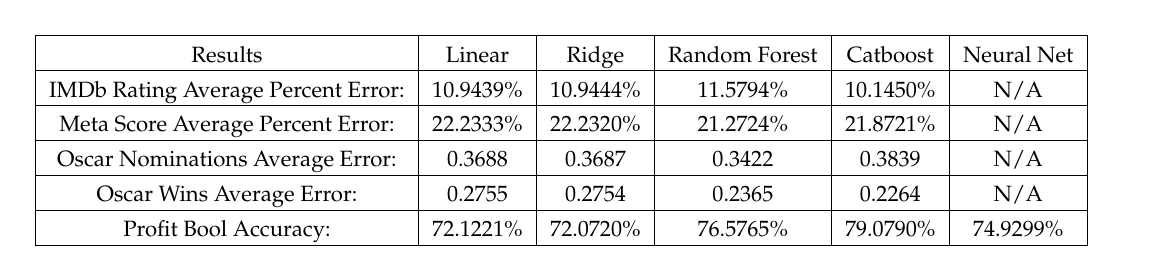
\begin{tikzpicture}
\node[rotate=0,scale=.8]{
\begin{tabular}{|c|c|c|c|c|c|c}
\cline{1-6}
Results & Linear & Ridge & Random Forest & Catboost & Neural Net & \rule{0pt}{2.6ex} \\
\cline{1-6}
IMDb Rating Average Percent Error: & 10.9439\% & 10.9444\% & 11.5794\% & 10.1450\% & N/A & \rule{0pt}{2.6ex} \\
\cline{1-6}
Meta Score Average Percent Error: & 22.2333\% & 22.2320\% & 21.2724\% & 21.8721\% & N/A & \rule{0pt}{2.6ex} \\
\cline{1-6}
Oscar Nominations Average Error: & 0.3688 & 0.3687 & 0.3422 & 0.3839 & N/A & \rule{0pt}{2.6ex} \\
\cline{1-6}
Oscar Wins Average Error: & 0.2755 & 0.2754 & 0.2365 & 0.2264 & N/A & \rule{0pt}{2.6ex} \\
\cline{1-6}
Profit Bool Accuracy: & 72.1221\% & 72.0720\% & 76.5765\% & 79.0790\% & 74.9299\% & \rule{0pt}{2.6ex} \\
\cline{1-6}
\end{tabular}};
\end{tikzpicture}
\]

After analyzing the results of all the machine learning algorithms implemented, it becomes apparent that determining the success of a movie is very difficult. Some characteristics of movies, such as word of mouth appeal, are very difficult to quantify. Including an actor network score into our models improved the accuracy of our predictions, however there are still many other variables to account for that detract from the accuracy. It is worth noting that every regressor model failed to accuractely estimate the profit a movie turned, because this value was extremely unpredicatable. Because Catboost was so fast and inherently more accurate, it enabled us to fine tune more than other models, to produce the most accurate predictions. Overall Catboost performed the best.
% Add a bibliography block to the postdoc

\hypertarget{references}{%
	\section{References}\label{references}}
\begin{description}

\item{[1]}\quad T., Michael, et al. “Early Predictions of Movie Success: the Who, What, and When of Profitability.” [1506.05382] Early Predictions of Movie Success: the Who, What, and When of Profitability, 29 Jan. 2016, arxiv.org/abs/1506.05382. 

\item{[2]}\quad University of California - Davis. "What Makes A Great Movie?." ScienceDaily. ScienceDaily, 16 August 2007. <www.sciencedaily.com/releases/2007/08/070815135034.htm>.

\item{[3]}\quad “Where Does the Information on IMDb Come from?” IMDb, IMDb.com, help.imdb.com/article/imdb/general-information/where-does-the-information-on-imdb-come-from/GGD7NGF5X3ECFKNN?ref\_=helpart\_nav\_22\#.
\end{description}
	
\end{document}


